\section{Reducció del temps}
Sí augmentem una barbaritat les iteracions, diguem 10000, el temps de càlcul augmenta, no linealment, sino exponencialment. \n
Això ho podem veure experimentalment:

\subsection{Per CPU}
Tractarem de paral·lelitzar amb la CPU. Tal i com he explicat abans, la CPU té diferents subprocessadors i els podem utilitzar tots a l'hora. \n
Utilitzarem la llibreria \emph{openmp}. És molt fàcil de fer servir, és una simple linea de codi i ajustar un parametre. \n
Aquí aniran algunes estimacions de quan de temps ens podem estalviar si utilitzaem la llibreria. \n
Amb aquesta llibreria no només paral·lelitzarem el càlcul de la fractal, també paral·lelitzarem el dibuix d'aquesta. Al fer-ho, tindrem una ventatge de - segons.

\subsection{Per GPU}
Aquesta paral·lelització disminuirà molt el temps de càlcul. Però no és tan senzill com la paral·lelització amb la CPU. \n
Utilitzarem CUDA, el qual ja no és una llibreria, si no és una extensió del lleguatge de programació C. Aquesta extensió ens permetrà accedir automàticament als subprocessadors. \n
Però no és tan senzill. Hi ha disponibles 1024 subprocessadors, els quals no és necessari utilitzar tots a l'hora però ho farem així perque volem la màxima eficiencia. \n
Tenim 1920x1080 punts. Hem d'accedir a cada un per saber la seva posició. Però no podem anar sumant 1 com feiem abans, perquè això només ho podem fer amb programació en serie. Per tant, el métode escollit serà aquest:
\begin{center}
    Si tenim 1024 subprocessadors i una graella d'\emph{AMPLADA}x\emph{ALTURA}, al total li direm $N$, per cada subprocessador agafarem un bucle que vagi fins a $N$ i començarem el bucle per l'identificador de cada subprocessador (ens donarà un nombre de l'1 al 1024), llavors, cada vegada que el bucle acabi, sumarem 1024. Així ens donarà un número únic en cada iteració del bucle i en cada subprocessador. Al fer aquest proscés, tindrem una graella semblant a aquesta (molt més gran, clar):
\end{center}

\centerline{
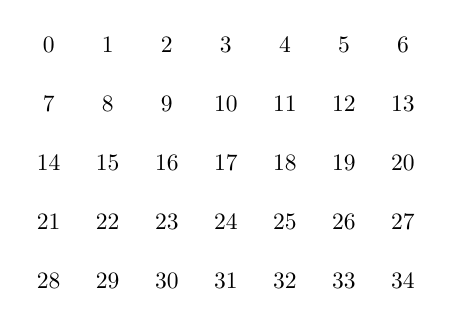
\begin{tikzpicture}
\foreach \x in {-2.25,-1.5,-0.75,0,0.75,1.5,2.25}
    \foreach \y in {-1.5,-0.75,0,0.75,1.5}
        \pgfmathtruncatemacro{\xy}{-(-\x*4/3+7*\y*4/3) + 17)}
        \draw (\x cm,\y cm) -- (\x cm,\y cm) node[anchor=center] {\scalebox{0.85}{\xy}};

\end{tikzpicture}
}

\begin{center}
    Agafarem el valor únic anterior i farem la divisió euclidiana, el divisor serà l'amplada, el quocient serà la posició $y$ i el residu la posició $x$. Això és més fàcil dir-ho que demostrar-ho. Per fer-ho, farem us de la graella anterior de 7x5.
\end{center}
\begin{center}
    Si ens hi fixem en un punt, diguem el 17, podem dir que el punt amb coordenades ($x$, $y$) és (2, 3), a ull, considerant el punt 0 com a (0, 0).
\end{center}
\centerline{
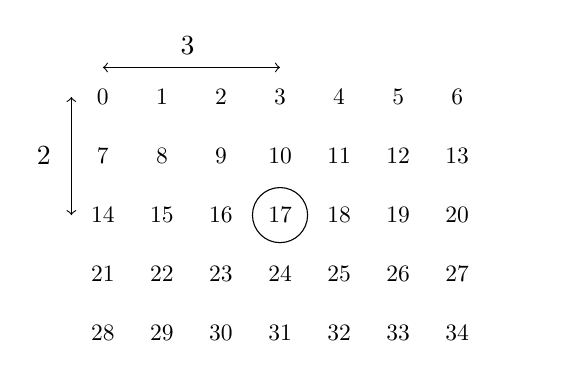
\begin{tikzpicture}
% El punt 17 té les coordenades:
% 0, 0

\draw [thin, to-to](-2.25,1.875) -- (0,1.875);
\draw [thin, to-to](-2.65,1.5) -- (-2.65,0);
\draw (0,0) circle (0.35);
\draw (-1.175, 2.15) node[anchor=center] {3};
\draw (-3, 0.75) node[anchor=center] {2};

\draw [thin, to-to, color=white](2.65,-1.5) -- (2.65,0);
\draw [color=white](3, -0.75) node[anchor=center] {2};


\foreach \x in {-2.25,-1.5,-0.75,0,0.75,1.5,2.25}
    \foreach \y in {-1.5,-0.75,0,0.75,1.5}
        \pgfmathtruncatemacro{\xy}{-(-\x*4/3+7*\y*4/3) + 17)}
        \draw (\x cm,\y cm) -- (\x cm,\y cm) node[anchor=center] {\scalebox{0.85}{\xy}};


\end{tikzpicture}
}

\begin{center}
    Podem veure que per passar una casella cap a baix, és a dir, augmentar la $y$ en 1, hem de sumar 7. Aquest 7 no és arbritari, és l'amplada. Si volem anar una casella amunt, disminuir la $y$ en 1, hem de restar 7, el que és el mateix l'amplada. En canvi, si volem moure'ns per les $x$\'s, llavors simplement hem d'augmentar o disminuir 1. Per tant, si dividim el nombre de la casella per l'amplada i obtenim el residu, obtenim el nombre en sí:
\end{center}

\centerline{\opidiv{17}{7}}

\begin{center}
    Com hem vist abans, el divisor és l'amplada, el quocient és l'ordenada $y$ i el residu l'ordenada $x$. S'ha de dir que aquest resultat no ens dona les coordenades en la fractal, si no ens dona en coordenades del cursor. Simplement ho passem per la funció creada anteriorment per passar-ho.
\end{center}

\noindent Les parts que es diferèncien del codi de CUDA i el codi amb C++ es troben a la pàgina \pageref{app:CUDA}, dins de l'Annex. \n
Amb CUDA no paral·lelitzarem el dibuix de la fractal, tal i com hem fet a l'anterior. Això és degut a que el temps de sincronització és més alt que el temps que el temps de càlcul en paral·lel amb la CPU. Així doncs, ho deixarem així. Per tant, mesclarem les dues i ens donarà el resultat més eficient. Sempre parlant de l'aplicació del conjunt de Mandelbrot. \n

\noindent En l'aplicació del conjunt de Julia, el càlcul en paral·lel, primerament no resulta beneficiòs. Ja que per comunicar amb la gràfica ja tarda més, en alguns casos, que el càlcul en serie.

\subsubsection{A vegades no és tan eficient, conjunt de Julia}
He recopilat algunes dades per veure aquesta pèrdua d'eficiéncia. Ja sabem què causa aquesta ineficiència però em resulta interessant comentar aquestes dades. \n
Les dades són el temps que tarda en fer el càlcul de la fractal i anem girant c. Tenim un total de 360 dades, una per cada grau que fem girar c. Aquesta comença amb una magnitud de ... i a 0 graus. Totes les dades es troben a l'Annex, pàgina \pageref{app:Julia_times}.
